\SourcePage{145}
\SGAsection{3}{孤立奇点}
\textbf{3.1. \Term{vanishing-cycle-manifold}{消失圈流形}。}

\textbf{3.1.1。}设 $D=\{z\in\mathbb C\mid |z|<1\}$，$X$ 为\Term{analytic-space}{解析空间}，$0\in X$，且 $f:X\to D$ 为满足 $f(0)=0$ 的\Term{morphism}{态射}。假设 $f$ 在 $0$ 之外\Term{smooth-morphism}{光滑}（特别地，$X$ 在 $0$ 之外\Term{smooth-morphism}{光滑}）。我们要研究 $0$ 附近的\Term{vanishing-cycles}{消失圈}；因此可以不失\Term{generic}{一般}性地假设 $X$ \Term{embedding}{嵌入} $\mathbb C^n\times D\subset\mathbb C^{n+1}$，\Term{embedding}{嵌入}与到 $D$ 的\Term{projection}{投影}相容，且将 $0$ 送到 $0$。

\textbf{3.1.2。}设 $\delta(x)$ 是 $X$ 上的实解析函数（即 $\mathbb C^{n+1}$ 上某个实解析函数在 $X$ 上的\Term{restriction}{限制}），对 $x\in X_0=f^{-1}(0)$ 满足
\[
\text{(a)}\quad\delta(x)\geq0;\qquad
\text{(b)}\quad\delta(x)=0\Longleftrightarrow x=0.
\]
例如可取 $\delta$ 为 $\mathbb C^{n+1}$ 中 $x$ 到 $0$ 的欧氏距离的平方。$\delta$ 在 $X_0$ 上的\Term{restriction}{限制}的\Term{critical-point}{临界点}\Term{set}{集合}是实解析的，因此在 $0$ 的适当\Term{neighbourhood}{邻域}内只有\Term{finite}{有限}多个\Term{connected-component}{连通分支}。将 $X$ 换成 $0$ 的一个开\Term{neighbourhood}{邻域}，并应用 Sard \Term{theorem}{定理}，就可以得到下列情形：
\[
\begin{array}{ll}
\text{(c)}&\text{对某个适当的 }r>0,\quad X_0\cap\delta^{-1}([0,r])\text{ 是紧的；}\\
\text{(d)}&\delta\text{ 在 }X_0\text{ 上没有小于或等于 }r\text{ 的临界值。}
\end{array}
\]
再适当缩小 $X$，还可以使：

(e) 存在 $C^\infty$ 函数 $\tau(s)$（$0\leq s\leq r$），满足 $\tau(0)=0$，且 $s>0$ 时 $\tau'(s)>0$；当 $0<s\leq r$、$0\leq |t|^2\leq\tau(s)$ 时，$X_t=f^{-1}(t)$ 与 $X$ 的实\Term{hypersurface}{超曲面} $\delta(x)=s$ \Term{transverse}{横截}，并且盒子
\[
 B_{t,d}=\{x\in X\mid \delta(x)\leq d\text{ 且 }|f(x)|^2<t\}
\]
到半径为 $t^{1/2}$ 的开\Term{disc}{圆盘} $D_t$ 的映射是\Term{proper-morphism}{固有的}。

\SourcePage{146}
令 $L=X_0\cap\delta^{-1}(r)$。由 (c)、(d)，$X_0\cap\delta^{-1}([0,r])$ 与锥
\[
 L\times[0,r]/\text{将 }L\times\{0\}\text{ 压缩为一点}
\]
之间存在一个\Term{homeomorphism}{同胚}，它将 $\delta$ 变为第二坐标，且在原点以外为 $C^\infty$。

\textbf{3.1.3。}设 $d\leq r$，$t\leq\tau(d)$。在 $0$ 之外，$B_{t,d}$ 是一个\Term{manifold-with-corners}{带角流形}，而 $B_{t,d}$ 到 $D_t$ 的\Term{projection}{投影} $f$ 是一个\Term{topological-fibration}{纤维化}。特别地：

(a) $B_{t,d}$ 在 $D_t^*=D_t-\{0\}$ 上诱导一个以紧\Term{manifold-with-boundary}{带边流形}为\Term{fibre}{纤维}的 $C^\infty$ \Term{fibre-bundle}{纤维丛}；

(b) 此\Term{fibre-bundle}{纤维丛}的\Term{boundary}{边界} $\delta(x)=d$ 延拓为 $D_t$ 上以紧\Term{manifold}{流形}为\Term{fibre}{纤维}的 $C^\infty$ \Term{fibre-bundle}{纤维丛} $\partial B_{t,d}$。

设 $y\in D_t^*$。称\Term{manifold-with-boundary}{带边流形} $V=f^{-1}(y)$ 为\Term{vanishing-cycle-manifold}{消失圈流形}。\Term{disc}{圆盘}是\Term{contractible}{可缩的}，故 $D_t$ 上的\Term{fibre-bundle}{纤维丛} $\partial B_{t,d}$ \Term{isomorphism}{同构}于\Term{fibre}{纤维}为 $\partial V$ 的常值\Term{fibre-bundle}{纤维丛}，且在 $y$ 上的\Term{fibre}{纤维}上为恒等的\Term{fibre-bundle}{纤维丛}\Term{isomorphism}{同构}
\[
 \partial B_{t,d}\xrightarrow{\sim}\partial V\times D_t
\]
的\Term{set}{集合}是\Term{contractible}{可缩的}。选取其中一个，记为 $\alpha$。将 $S_{|y|}$（半径为 $|y|$ 的圆周）上的\Term{vector-field}{向量场} $\partial/\partial\theta$ \Term{lifting}{提升}为 $f^{-1}(S_{|y|})$ 上的\Term{vector-field}{向量场} $u$，使其在\Term{boundary}{边界}上与 $\alpha$ 相容，即
\[
 d\alpha(u)=(\partial/\partial\theta,0).
\]
这些\Term{lifting}{提升}的\Term{set}{集合}是\Term{contractible}{可缩的}。对 $u$ 积分（沿正向转一圈），就得到 $V$ 的一个\Term{diffeomorphism}{微分同胚} $T$，它在 $\partial V$ 上为恒等；这就是\Term{monodromy-transformation}{单值变换}。模去相对于 $\partial V$ 的\Term{isotopy}{同痕}后，它是良定义的。

在一种留给读者确切表述的意义下，$(V,T)$ 与 $t$、$s$ 的选择无关。我不知道它是否与 $\delta$ 的选择无关。不过可以验证，若只允许取下述类型的 $\delta$，则确实无关：$\delta$ 是 $\mathbb C^{n+1}$ 上某个函数 $f$ 在 $X$ 上的\Term{restriction}{限制}，且在 $X_0$ 于 $0$ 的 Zariski \Term{tangent-space}{切空间}上满足 $df=0$、$d^2f>0$（\Term{positive-definite}{正定}）。关键在于，对这种类型的 $\delta$ 和 $\delta'$，可以对所有 $\lambda\delta+(1-\lambda)\delta'$（$0\leq\lambda\leq1$）一致地选取满足 3.1.2 (c)、(d) 的 $r$。

\textbf{3.1.4。}设 $(V_1,T_1)$ 由 $(V,T)$ 添加一个领圈而得：
\SourcePage{147}
\[
 V_1-V^\circ\simeq\partial V\times[0,1],\qquad
 T_1\text{ 在 }V_1-V^\circ\text{ 上为恒等。}
\]
令 $f':W\to D_t$ 为 $D_t$ 上的如下\Term{space}{空间}（参见 1.4.3）：

(a) 设 $\widetilde D_t^*$ 是以 $y$ 为\Term{base-point}{基点}的 $D_t^*$ 的\Term{universal-covering}{万有覆盖}；$W^*$ 为 $D_t^*$ 上的\Term{fibre-bundle}{纤维丛}，由 $V_1\times\widetilde D_t^*$ 对下述关系所生成的\Term{equivalence-relation}{等价关系}取商而成：
\[
 (v,y)\sim(T_1v,e^{2\pi i}y).
\]
(b) 因为 $T_1|_{V_1-V^\circ}$ 是恒等，可以将 $W^*$ 与 $D_t$ 上\Term{fibre}{纤维}为 $V_1-V$ 的\Term{trivial-bundle}{平凡丛}\Term{gluing}{粘合}，得到 $D_t$ 上的\Term{space}{空间} $W_1$。

(c) $W=W_1\cup\{0\}$，$f'(0)=0$。赋予 $W$ 唯一的\Term{topology}{拓扑}，使它诱导 $W_1$ 原有的\Term{topology}{拓扑}，使 $f'$ \Term{continuous}{连续}，并使 $f'^{-1}(\overline D_{t'})$（$t'<t$）为 $W_1\cap f'^{-1}(\overline D_{t'})$ 的单点\Term{compactification}{紧化}。

在 $W-\{0\}$ 上赋予这样的\Term{integrable-connection}{可积联络}（1.3.4）：由 (a) 给出的、$W$ 在 $\widetilde D_t^*$ 上的\Term{inverse-image}{逆像}的\Term{trivialization}{平凡化}是水平的。

\begin{SGAresult}{命题}{3.1.5}
存在 $B_{s,t}$ 与 $W$ 之间的\Term{homeomorphism}{同胚} $\psi$，它与到 $D_t$ 的\Term{projection}{投影}相容，并将 $0$ 送到 $0$；还可以使这个\Term{homeomorphism}{同胚}在 $0$ 之外为\Term{diffeomorphism}{微分同胚}。
\end{SGAresult}

这一结果在本讨论班后文中不会用到。

\begin{proof}
设 $d_0<d_1\leq r$，$t_0\leq\tau(d_0)$，且 $y\in D_{t_0}^*$。有 $B_{t_0,d_0}\subset B_{t_0,d_1}$，而 $B_{t_0,d_1}-B_{t_0,d_0}^\circ$ 是 $D_{t_0}$ 上的\Term{fibre-bundle}{纤维丛}。将它\Term{trivialization}{平凡化}，并在圆周 $S_{|y|}$ 上以与该\Term{trivialization}{平凡化}相容的方式\Term{lifting}{提升}\Term{vector-field}{向量场} $\partial/\partial\theta$。令 $T_1$ 为所得的 $V_1=f^{-1}(y)\cap B_{t_0,d_1}$ 的\Term{endomorphism}{自同态}，且令 $V_0=f^{-1}(y)\cap B_{t_0,d_0}$。于是 $(V_0\subset V_1,T_1)$ \Term{isomorphism}{同构}于 3.1.4 中的 $(V\subset V_1,T_1)$。利用 $(V_0\subset V_1,T_1)$ 构造 $W$，便有\Term{canonical}{典范}等式 $f'^{-1}(y)=V_1$。证明将表明，可以选取 $\psi$ 使它诱导\Term{identity-map}{恒等映射} $f^{-1}(y)\xrightarrow{\sim}f'^{-1}(y)$。

下图（$f$ 及其在 $f^{-1}(\mathbb R)$ 上的\Term{restriction}{限制}）概括了证明：
\SourcePage{148}
\begin{center}
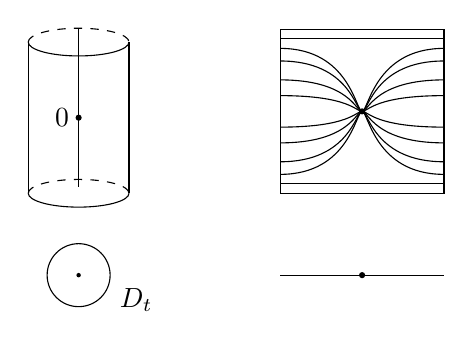
\begin{tikzpicture}[scale=.8]
\draw (0,0) arc[start angle=180,end angle=360,x radius=.8,y radius=.22];
\draw[dashed] (0,0) arc[start angle=180,end angle=0,x radius=.8,y radius=.22];
\draw (0,0)--(0,2.4) (1.6,0)--(1.6,2.4);
\draw (0,2.4) arc[start angle=180,end angle=360,x radius=.8,y radius=.22];
\draw[dashed] (0,2.4) arc[start angle=180,end angle=0,x radius=.8,y radius=.22];
\draw (.8,.1)--(.8,2.6);\fill (.8,1.2) circle(1.4pt);\node[left] at (.8,1.2){$0$};
\draw (.8,-1.3) circle(.5);\fill (.8,-1.3) circle(1pt);\node[right] at (1.3,-1.7){$D_t$};
\draw (4,0) rectangle (6.6,2.6);\draw (4,2.45)--(6.6,2.45) (4,.15)--(6.6,.15);
\foreach \a in {.3,.5,.8,1.05}{\draw (4,\a) .. controls (5.1,\a) and (5.2,1.3) .. (5.3,1.3) .. controls (5.4,1.3) and (5.5,\a) .. (6.6,\a);\draw (4,{2.6-\a}) .. controls (5.1,{2.6-\a}) and (5.2,1.3) .. (5.3,1.3) .. controls (5.4,1.3) and (5.5,{2.6-\a}) .. (6.6,{2.6-\a});}
\fill (5.3,1.3) circle(1.4pt);\draw (4,-1.3)--(6.6,-1.3);\fill (5.3,-1.3) circle(1.4pt);
\end{tikzpicture}
\end{center}

设 $B^+\subset B_{t_0,d_1}$ 由满足 $|f(x)|^2\leq\tau(\delta(x))$ 的 $x$ 构成。取一列从 $[0,t_0]$ 到 $(0,d_1]$ 的 $C^\infty$ 函数 $\varphi_n$，使得对某列趋于 $0$ 的数 $r_0>r_1>\cdots$，有：

(a) 当 $|t|^2\geq r_i$ 时，$\varphi_i$ 为 $\tau$ 的反函数；

(b) 当 $|t|^2<r_i$ 且 $j>i$ 时，$\varphi_j(t)<\varphi_i(t)$。
\begin{center}
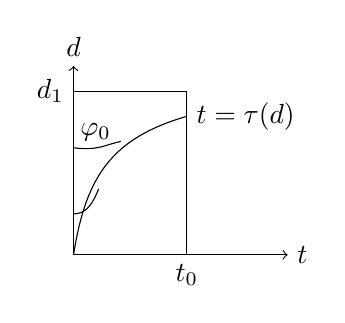
\begin{tikzpicture}[scale=.8]
\draw[->] (0,0)--(3.4,0) node[right]{$t$};\draw[->] (0,0)--(0,3) node[above]{$d$};
\draw (0,2.6) node[left]{$d_1$}--(1.8,2.6)--(1.8,0) node[below]{$t_0$};
\draw (0,0) .. controls (.2,1.25) and (.6,1.85) .. (1.8,2.2) node[right]{$t=\tau(d)$};
\draw (0,1.7) .. controls (.4,1.65) and (.5,1.75) .. (.75,1.8);\node at (.35,1.95){$\varphi_0$};
\draw (0,.65) .. controls (.2,.65) and (.3,.8) .. (.4,1.05);
\end{tikzpicture}
\end{center}
$B^+-\{0\}$ 是 $D_t$ 上的\Term{fibre-bundle}{纤维丛} $B_i^+$ 的并，其中
\[
 B_i^+:\quad\delta(x)\geq\varphi_i(|f(x)|^2).
\]
利用 $\delta$ 在 $B^+-\{0\}\to D_t$ 的\Term{fibre}{纤维}上没有\Term{critical-point}{临界点}，由一个标准论证可知，存在 $B_i^+$ 到 $B_{i+1}^+$ 的\Term{diffeomorphism}{微分同胚} $\alpha_i$，它与到 $D_t$ 的\Term{projection}{投影}相容，并在 $B_i^+$ 的\Term{vector-subspace}{子空间}
\SourcePage{149}
\[
 \{\delta(x)=\varphi_i(|f(x)|^2),\ |f(x)|^2\leq r_i\}
\]
的一个小\Term{neighbourhood}{邻域}之外为恒等。将各 $\alpha_i$ 复合并取\Term{limit}{极限}，就得到
\[
 B_0^+-\{x\mid f(x)=0\text{ 且 }\delta(x)=\varphi_0(0)\}
 \xrightarrow[\alpha]{\sim} B^+-\{0\}
\]
的\Term{diffeomorphism}{微分同胚}。利用 $\alpha$ 搬运 $D_t$ 上的\Term{fibre-bundle}{纤维丛} $B_0^+$ 的一个\Term{trivialization}{平凡化}，就得到 $B^+-\{0\}$ 上的\Term{integrable-connection}{可积联络} $\nabla'$。于是可以：

(a) 将该\Term{connection}{联络}在 $f^{-1}(S_{|y|})\cap B^+$ 上的\Term{restriction}{限制}延拓为 $f^{-1}(S_{|y|})/S_{|y|}$ 上的\Term{connection}{联络}（这个延拓给出 $T_1$）；

(b) 将 $\nabla'$ 所给出的 $D_t$ 上径向\Term{vector-field}{向量场}在 $B^+-\{0\}$ 上的\Term{lifting}{提升}延拓到 $B_{t_0,d_1}$。

于是 $B_{t_0,d_1}$ 上存在唯一的\Term{integrable-connection}{可积联络} $\nabla$，它延拓 $\nabla'$、(a) 和 (b)；并存在唯一的水平\Term{diffeomorphism}{微分同胚} $B_{t_0,d_1}-\{0\}\xrightarrow{\sim}W-\{0\}$，在 $f^{-1}(y)$ 上为恒等。这就解决了问题。
\end{proof}

\textbf{3.1.6. 一个推广。}以上讨论可推广到这样的\Term{morphism}{态射} $f:X\to D$：$0\in X$ 是 $X_0$ 中的一个孤立的非\Term{smooth-morphism}{光滑}点。适当缩小 $X$ 和 $D$ 后，$f$ 的非\Term{smooth-morphism}{光滑}点集在 $D$ 上是\Term{finite}{有限}的。此时\Term{vanishing-cycle-manifold}{消失圈流形} $V$ 有一个\Term{finite}{有限}\Term{critical-point}{临界点}集 $\Sigma$；$V-\Sigma$ 是\Term{manifold-with-boundary}{带边}\Term{differentiable-manifold}{微分流形}（\Term{boundary}{边界}紧，但自身不紧）。\Term{monodromy-transformation}{单值变换} $T$ 在\Term{boundary}{边界}上为恒等，并保持 $\Sigma$ \Term{invariant}{不变}。最后，3.1.5 仍然成立：该\Term{fibre-bundle}{纤维丛}\Term{homeomorphism}{同胚} $\psi$ 在\Term{critical-point}{临界点}集之外是\Term{diffeomorphism}{微分同胚}，并将\Term{critical-point}{临界点}集送到 $W$ 中来自 $\Sigma$ 的部分。

\textbf{3.1.7。}命题 3.1.5 使我们可以运用 1.4 的计算，从而得到：

(A) \Term{vanishing-cycles}{消失圈}群 $(R^i\Phi(\Lambda))_0$ 是\Term{vanishing-cycle-manifold}{消失圈流形} $V$ 的、取值于 $\Lambda$ 的\Term{reduced-cohomology}{约化上同调}群。

(B) 群 $H_{\{0\}}^i(X_0,R\Psi(\Lambda))$ 是 $V^\circ$ 的、取值于 $\Lambda$ 的\Term{proper-support}{固有支撑}\Term{cohomology}{上同调}群。

(C) \Term{variation}{变差}
\SourcePage{150}
\[
 \operatorname{Var}:\widetilde H^i(V,\Lambda)\longrightarrow H_c^i(V^\circ,\Lambda)
 =H^i(V\bmod\partial V,\Lambda)
\]
就是由 $V$ 的\Term{automorphism}{自同构} $T$（在 $\partial V$ 上为恒等）定义的经典\Term{variation}{变差}。

\textbf{3.1.8。}事实上，断言 (A)、(B)、(C) 比 3.1.5 更为初等。下面给出一个直接的证明与构造，从而无需再验证\Term{isomorphism}{同构} (A)、(B) 与构造 3.1.5 中所作的选择无关。

设 $d\leq r$，$t\leq\tau(d)$，且 $B$ 为开盒子
\[
 B=\{x\mid\delta(x)<d\text{ 且 }|f(x)|^2<t\}.
\]
设 $\widetilde D^*$ 为 $D^*$ 的\Term{universal-covering}{万有覆盖}，并令
\[
\begin{tikzcd}
\{0\}\arrow[r,hook,"\bar i"]\arrow[d,equal]&\overline D_t\arrow[d,"p"]&\widetilde D_t^*\arrow[l,"\bar j"']\arrow[d,"p'"]\\
\{0\}\arrow[r,hook,"i"]&D_t&D_t^*\arrow[l,hook,"j"']
\end{tikzcd}\tag{3.1.8.1}
\]
为将 1.2.7.2 \Term{restriction}{限制}到 $D_t$ 所得的图。令
\[
\begin{tikzcd}
 B_0\arrow[r,hook,"\bar i"]\arrow[d,equal]&\overline B\arrow[d,"p"]&\overline B^*\arrow[l,"\bar j"']\arrow[d,"p'"]\\
 B_0\arrow[r,hook,"i"]&B&B^*\arrow[l,hook,"j"']
\end{tikzcd}\tag{3.1.8.2}
\]
为 $f:B\to D$ 在 (3.1.8.1) 上的\Term{inverse-image}{逆像}。仍以 $f$ 表示 (3.1.8.2) 到 (3.1.8.1) 的\Term{projection}{投影}。

(A) 由定义，$R^i\Psi_\eta(\Lambda)_0$ 是当 $U$ 遍历 $X$ 中 $0$ 的\Term{neighbourhood}{邻域}时，\Term{cohomology}{上同调}群 $H^i(U\times_D\widetilde D^*,\Lambda)$ 的\Term{direct-limit}{归纳极限}。让 $U$ 遍历由上述盒子 $B$ 构成的 $0$ 的\Term{neighbourhood-basis}{邻域基}。\Term{fibre-product}{纤维积} $U\times_D\widetilde D^*=\overline B^*$ 是\Term{contractible}{可缩}\Term{space}{空间} $\widetilde D_t^*$ 上以 $V^\circ$ 为\Term{fibre}{纤维}的\Term{fibre-bundle}{纤维丛}。因此 $H^i(\overline B^*,\Lambda)$ 构成的\Term{inductive-system}{归纳系}是常值的，其值为 $H^i(V^\circ,\Lambda)=H^i(V,\Lambda)$。
\SourcePage{151}
所得\Term{isomorphism}{同构}
\[
 R^i\Psi_\eta(\Lambda)_0=H^i(V,\Lambda)\tag{3.1.8.3}
\]
可以细化为如下复合\Term{isomorphism}{同构}（参见下文 (B)）：
\begin{equation}
\begin{aligned}
 R\Psi_\eta(\Lambda)_0
 &\xleftarrow{\sim}R\Gamma(B_0,R\Psi_\eta(\Lambda))
 \xleftarrow{\sim}(Rf_*R\bar j_*\Lambda)_0
 \xleftarrow{\sim}R\Gamma(\overline D_t,Rf_*R\bar j_*\Lambda),\\
 R\Gamma(V,\Lambda)&\xrightarrow{\sim}R\Gamma(V^\circ,\Lambda)
 \xleftarrow{\sim}R\Gamma(\overline B^*,\Lambda).
\end{aligned}\tag{3.1.8.4}
\end{equation}
这里两行右端之间为\Term{canonical}{典范}\Term{isomorphism}{同构}。\Term{complex}{复形} $R\Phi(\Lambda)_0$ 由\Term{distinguished-triangle}{区别三角}
\[
 \Lambda\longrightarrow(R\Psi_\eta\Lambda)_0\longrightarrow R\Phi(\Lambda)_0\longrightarrow
\]
定义。因此 $R^i\Phi(\Lambda)_0$ 就是 $V$ 的\Term{reduced-cohomology}{约化上同调}群。

(B) 设 $\Phi$ 为 $\overline B^*$ 中满足下述条件的\Term{closed-subset}{闭集}族：它在 $\overline B$ 中的\Term{closure}{闭包}在 $\overline D$ 上\Term{proper-morphism}{固有}。下列\Term{arrow}{箭头}都是\Term{isomorphism}{同构}：
\[
\begin{tikzcd}[column sep=large]
 R\Gamma_{\{0\}}(R\Psi_\eta(\Lambda))\arrow[r,"\sim\ (1)"]&R\Gamma_c(B_0,R\Psi_\eta(\Lambda))\arrow[r,"\sim\ (2)"]&(Rf_!R\bar j_*\Lambda)_0\\
 R\Gamma_c(V^\circ,\Lambda)&R\Gamma_\Phi(\overline B^*,\Lambda)\arrow[l,"\sim\ (5)"]&R\Gamma(\overline D_t,Rf_!R\bar j_*\Lambda)\arrow[u,"\sim\ (3)"']\arrow[l,equal,"(4)"]
\end{tikzcd}\tag{3.1.8.5}
\]
其中：(1) 因为 $B_0$ 是锥（3.1.2），且 $R^i\Psi_\eta(\Lambda)$ 在 $0$ 之外为常值；(2) 由\Term{proper-support}{固有支撑}\Term{direct-image}{正像}的\Term{base-change}{换基}\Term{theorem}{定理}；(3) 因为 $Rf_!R\bar j_*\Lambda$ 在 $0$ 之外为常值；(4) 是复合\Term{functor}{函子}\Term{spectral-sequence}{谱序列}的“\Term{derived-category}{导出范畴}”版本；(5) 因为 $\widetilde D^*$ 是\Term{contractible}{可缩的}。

\Term{isomorphism}{同构} (3.1.8.5) 给出所需的\Term{isomorphism}{同构}
\SourcePage{152}
\[
 R^i\Gamma_{\{0\}}(R\Psi_\eta(\Lambda))=H_c^i(V^\circ,\Lambda).\tag{3.1.8.6}
\]
我们将在 3.1.10 验证 (C)。

\textbf{3.1.9。}（参见 [3]。）设 $X$ 为\Term{topological-space}{拓扑空间}，$i:Y\hookrightarrow X$ 是 $X$ 的一个\Term{closed-subset}{闭子集}，$T$ 是 $X$ 的\Term{automorphism}{自同构}，在 $Y$ 上诱导恒等，且 $\Lambda$ 为\Term{abelian-group}{阿贝尔群}。为定义\Term{variation}{变差} $\operatorname{Var}$，选取 $X$ 上 $\Lambda$ 的一个 $T$-\Term{equivariant}{等变}\Term{resolution}{解消} $\Lambda_X^*$、$Y$ 上\Term{sheaf}{层} $\Lambda$ 的一个\Term{resolution}{解消} $\Lambda_Y^*$（约定 $T$ 在其上\Term{trivial-action}{平凡作用}），以及一个\Term{equivariant}{等变}\Term{morphism}{态射}
\[
 \varphi:\Lambda_X^*\longrightarrow i_*\Lambda_Y^*,
\]
它\Term{resolution}{解消}显然的\Term{morphism}{态射} $\varphi_0:\Lambda_X\to i_*\Lambda_Y$。假设\Term{sheaf}{层} $\Lambda_X^i$、$\Lambda_Y^i$ 对将要考虑的\Term{functor}{函子}都是\Term{acyclic}{无上同调的}。取\Term{global-section}{整体截面}得到
\[
 \Gamma(\varphi):\Gamma(\Lambda_X^*)\longrightarrow\Gamma(\Lambda_Y^*).
\]
为简单起见，假设各 $\Gamma(\varphi)^i$ 都\Term{surjective}{满射}（否则，可在 $\Gamma(\Lambda_X^*)$ 上添加 $\Gamma(\Lambda_Y^*)$ 的锥使其成为\Term{surjective}{满射}）。置
\[
 R\Gamma(X\bmod Y,\Lambda)=\operatorname{Ker}(\Gamma(\varphi)).
\]
在合理的假设下，若 $\Phi$ 是 $X$ 中与 $Y$ 不交的\Term{closed-subset}{闭集}族，则有\Term{quasi-isomorphism}{拟同构}
\[
 \Gamma_\Phi(X-Y,\Lambda_X^*)\xrightarrow{\sim}R\Gamma(X\bmod Y,\Lambda).
\]
$\Gamma(\Lambda_X^*)$ 的\Term{endomorphism}{自同态} $T-1$（$T$ 通过\Term{transport-of-structure}{结构搬运}\Term{action}{作用}）在 $\Lambda$（常数）上为零，并经由 $\operatorname{Ker}(\Gamma(\varphi))$ \Term{resolution}{分解}。因此，在同样的假设下，\Term{derived-category}{导出范畴}中有一个\Term{variation}{变差}\Term{morphism}{态射}
\[
 \operatorname{Var}:R\widetilde\Gamma(X,\Lambda)\longrightarrow R\Gamma_\Phi(X-Y,\Lambda)
\]
\SourcePage{153}
（不加假设时，则得到 $\operatorname{Var}:R\widetilde\Gamma(X,\Lambda)\to R\Gamma(X\bmod Y,\Lambda)$）。

若 $T$ 在 $Y$ 的一个\Term{neighbourhood}{邻域}内为恒等，并且在此\Term{neighbourhood}{邻域}内在 $\Lambda_X^*$ 上也为恒等，上述描述就更简单。此时 $\Gamma(\Lambda_X^*)$ 的\Term{endomorphism}{自同态} $T-1$ 经由 $\Gamma_\Phi(\Lambda_X^*)$ \Term{resolution}{分解}，从而给出\Term{variation}{变差}。

\begin{SGAresult}{命题}{3.1.10}
通过 3.1.8 (A)、(B) 的\Term{isomorphism}{同构}，\Term{variation}{变差}
\[
 (R\Phi_\eta(\Lambda))_0\longrightarrow R\Gamma_{\{0\}}(R\Psi_\eta(\Lambda))
\]
等于 3.1.9 中由 $V$ 的\Term{automorphism}{自同构} $T$（在 $\partial V$ 上为恒等）所定义的\Term{variation}{变差}。
\end{SGAresult}

\begin{proof}
建议读者画一幅小图来理解，而不必阅读以下证明。设 ${}_fB$ 为 3.1.2 的闭盒子，${}_fC\subset{}_fB$ 为沿\Term{boundary}{边界}的一个领圈（作为 $D_t$ 上的\Term{fibre-bundle}{纤维丛}，有 ${}_fC\simeq\partial{}_fB\times[0,1]$，此\Term{isomorphism}{同构}将 $\partial{}_fB\times\{1\}$ 恒等地送到 $\partial{}_fB$）。设
\[
 {}_f\alpha:{}_fC\xrightarrow{\sim}(\partial V\times[0,1])\times D_t
\]
为 $D_t$ 上的\Term{fibre-bundle}{纤维丛} ${}_fC$ 的一个\Term{trivialization}{平凡化}，使它在 $y\in D_t$ 处的\Term{fibre}{纤维}诱导\Term{identity-map}{恒等映射} $\partial V=\partial(f^{-1}(y))\xrightarrow{\sim}\partial V\times\{1\}$。令 $C={}_fC\cap B$，并令
\[
 \alpha:C\xrightarrow{\sim}(\partial V\times[0,1[)\times D_t
\]
为 ${}_f\alpha$ 诱导的映射。沿用 3.1.8.2 的记号。

令 $R$ 为 $\overline B$ 上的\Term{equivalence-relation}{等价关系}：
\[
 x=y\quad\text{或}\quad p(x),p(y)\in C\text{ 且 }\alpha(p(x)),\alpha(p(y))
 \text{ 在 }\partial V\times[0,1[\text{ 中有相同的像。}
\]
令 ${}_1\overline B=\overline B/R$、${}_1\overline B^*=\overline B^*/R$、${}_1\overline C^*=p^{-1}(C)/R$。有如下\Term{commutative-diagram}{交换图}：
\SourcePage{154}
\[
\begin{tikzcd}
 B_0\arrow[r,hook,"\bar i"]\arrow[d,equal]&\overline B\arrow[d,"q"]&\overline B^*\arrow[l,"\bar j"']\arrow[d,"q'"]\\
 B_0\arrow[r,hook,"\bar i"]&{}_1\overline B&{}_1\overline B^*\arrow[l,"{}_1\bar j"']
\end{tikzcd}
\]
设 $\Lambda^*$ 为 $\overline B^*$ 上由\Term{acyclic}{无上同调}\Term{sheaf}{层}构成的 $\pi_1(D^*)$-\Term{equivariant}{等变}\Term{resolution}{解消}。由定义，\Term{variation}{变差}可从\Term{complex}{复形}\Term{morphism}{态射}
\[
 \Lambda[0]\longrightarrow\bar i^*\bar j_*(\Lambda^*)
\]
算出。因为 $\Lambda\xrightarrow{\sim}Rq_*\Lambda$ 且 $\Lambda\xrightarrow{\sim}Rq'_*\Lambda$，也可以利用 ${}_1\overline B^*$ 上 $\Lambda$ 的一个\Term{equivariant}{等变}\Term{resolution}{解消}和\Term{morphism}{态射}
\[
 \Lambda[0]\longrightarrow\bar i^*{}_1\bar j_*(\Lambda)
\]
来计算它。

通过 (A)、(B)，\Term{variation}{变差}由此等同于复合\Term{morphism}{态射}
\[
\begin{tikzcd}[column sep=large]
 R\Gamma(V,\Lambda)\arrow[r,"\sim"]&R\Gamma(V^\circ,\Lambda)&R\Gamma({}_1\overline B^*,\Lambda)\arrow[l,"\sim\ (1)"']\arrow[d,"\operatorname{Var}"]\\
 &R\Gamma_c(V^\circ,\Lambda)&R\Gamma({}_1\overline B^*\bmod{}_1\overline C^*,\Lambda)\arrow[l,"\sim\ (2)"]
\end{tikzcd}\tag{3.1.10.1}
\]
其中 (1)、(2) 由 $V^\circ$ 到 ${}_1\overline B^*$ 的包含诱导，而 $\operatorname{Var}$ 为 3.1.9 中对 ${}_1\overline B^*$ 及 $\pi_1(D^*)$ 的正\Term{generator}{生成元}\Term{action}{作用}所定义的\Term{variation}{变差}（此群通过其 1.1.5 中的\Term{action}{作用}在 ${}_1\overline B^*$ 上\Term{action}{作用}；在 ${}_1\overline C^*$ 上则\Term{trivial-action}{平凡作用}）。

选取 $B^*/D^*$ 上的一个\Term{connection}{联络} $\nabla$，与 $C$ 的\Term{trivialization}{平凡化}相容。这个\Term{connection}{联络}将 $\overline B^*$ \Term{trivialization}{平凡化}，并经取商给出 $u:{}_1\overline B^*\to V$。对按 3.1.3 定义的 $T$，图
\SourcePage{155}
\[
\begin{tikzcd}
 {}_1\overline B^*\arrow[r,"u"]\arrow[d,"T"']&V\arrow[d,"T"]\\
 {}_1\overline B^*\arrow[r,"u"]&V
\end{tikzcd}
\]
交换。映射 $u$ 诱导\Term{cohomology}{上同调}的\Term{isomorphism}{同构}，故 (3.1.10) 由 3.1.10.1 和\Term{variation}{变差}的\Term{functoriality}{函子性}得出。
\end{proof}

命题 3.1.10 将用来说明我们稍后的一项显式计算为何成立。在那里，与此处一样，$T$ 在 $\partial V$ 的一个\Term{neighbourhood}{邻域}内为恒等。我们将取一个由流 $C$ 表示的\Term{cohomology}{上同调}类 $c$，并利用 $\operatorname{Var}(c)$ 由在 $V^\circ$ 中具有紧\Term{support}{支撑}的流 $TC-C$ 表示这一事实。

\textbf{3.1.11。}实际计算 $T$ 时，常分两步进行：

(a) 固定 $t$、$d$，使 $t\leq\tau(d)$；选取 $y\in D_t$，并在 $f^{-1}(S_{|y|})\cap B_{t,d}$ 上选取\Term{connection}{联络} $\nabla$。它给出 $V_0=f^{-1}(y)\cap B_{t,d}$ 的一个\Term{diffeomorphism}{微分同胚} $T_0$，但 $T_0$ 在\Term{boundary}{边界}上未必为恒等。

(b) 选取 $D_t$ 上 $\partial B_{t,d}$ 的一个\Term{trivialization}{平凡化}。对 $\nabla$ 积分给出 $\partial V$ 到 $f^{-1}(e^{2\pi i\theta}y)\cap\partial B_{t,d}$ 的\Term{diffeomorphism}{微分同胚} $\varphi(\theta)$，而后者由\Term{trivialization}{平凡化}等同于 $\partial V$。当 $0\leq\theta\leq1$ 时，$\varphi(\theta)$ 是 $\operatorname{Diff}(\partial V)$ 中一条连接恒等与 $\partial T_0$ 的\Term{path}{路径}。

得到的二元组 $(T_0,\varphi)$ 依赖于所作的任意选择。由于这些选择的\Term{set}{集合}是\Term{contractible}{可缩的}，模去\Term{homotopy}{同伦}后便与选择无关。对 3.1.3 类型的 $T$，$(T,\text{常值路径})$ 就是这里所考虑类型的一个 $(T_0,\varphi)$。

\textbf{3.1.12。}已知 $\operatorname{Diff}(V)\to\operatorname{Diff}(\partial V)$ 是\Term{topological-fibration}{纤维化}，因此 $T\mapsto(T,\text{常值路径})$ 在下列两者间诱导一个\Term{bijection}{双射}：

(a) 满足 $\partial T=\operatorname{Id}$ 的\Term{diffeomorphism}{微分同胚} $T:V\to V$ 的\Term{set}{集合}，模去\Term{isotopy}{同痕}；
\SourcePage{156}
(b) 二元组 $(T_0,\varphi)$ 的\Term{set}{集合}，其中 $T_0:V\xrightarrow{\sim}V$，$\varphi$ 是从 $\operatorname{Id}$ 到 $\partial T_0$ 的\Term{path}{路径}的\Term{homotopy}{同伦}类，再模去\Term{isotopy}{同痕}。

故由上面的 (a)、(b) 算出的一个二元组 $(T_0,\varphi)$ 就确定了 $T$。具体地，可以如下由 $(T_0,\varphi)$ 算出 $T$：

($\alpha$) 在 $V$ 中取 $\partial V$ 的一个领圈 $[0,1]\times\partial V\xrightarrow{\alpha}V$（$\alpha(1,x)=x$），并选取 $\varphi$ 的代表元，使 $\varphi:[0,1]\to\operatorname{Diff}(\partial V)$ 在 $x<0$ 时延拓为恒等后是 $C^\infty$ 的。在此领圈内，令 $\beta(x)=\operatorname{pr}_1\alpha^{-1}(x)$（$\beta$ 无\Term{critical-point}{临界点}，取值于 $[0,1]$，且在 $\partial V$ 上等于 $1$）。

($\beta$) 在领圈以外取 $T=T_0$，而在领圈内取
\[
 T(x)=T_0\bigl(\varphi(\beta(x))^{-1}(x)\bigr).
\]

\textbf{3.1.13。}下面是 3.1.11 (b) 的一个变体，用来计算\Term{path}{路径} $\varphi$ 的\Term{homotopy}{同伦}类。在每条射线 $\arg(z)=\theta$ 上，选取\Term{fibre-bundle}{纤维丛} $\partial B_{t,d}$ 的一个\Term{trivialization}{平凡化}，使它随 $\theta$ \Term{continuous}{连续}变化。利用通过 $y$ 的射线上方的\Term{trivialization}{平凡化}，将 $(\partial V)_0=f^{-1}(0)\cap\partial B_{t,d}$ 等同于 $\partial V$。设 $\psi_\theta:V\to f^{-1}(e^{i\theta}y)\cap B_{t,d}$ 由对 $\nabla$ 积分而得。将射线搬运到 $\psi_\theta$，得到 $(\partial V)_0$、从而 $\partial V$ 的一个\Term{diffeomorphism}{微分同胚}。它就是 $\varphi(\theta)$。

\textbf{3.2. \Term{picard-lefschetz-formula}{Picard--Lefschetz 公式}（\Term{transcendental}{超越}情形）。}

\textbf{3.2.1。}我们要对从 $\mathbb C^{n+1}$ 到 $\mathbb C$ 的映射 $f=\sum_{1}^{n+1}z_i^2$ 显式写出 3.1 的结果。取 $\delta=\sum|z_i|^2$，并取盒子 $B=B_{a,b}$：
\[
 \left|\sum z_i^2\right|\leq a^2,\qquad\sum|z_i|^2\leq b^2,
\]
其中 $0<a<b$（取闭盒子而非 3.1.2 的盒子，只是为了简化记号）。
\SourcePage{157}
\textbf{3.2.2。}\Term{vanishing-cycle-manifold}{消失圈流形} $V$ 的方程为
\[
 \sum z_i^2=a^2,\qquad\sum|z_i|^2\leq b^2.\tag{3.2.2.1}
\]
将 $z=(z_i)$ \Term{resolution}{分解}为实部与虚部：$z=x+iy$。上述方程改写为
\[
 x^2-y^2=a^2,\qquad x\cdot y=0\quad(\text{即 }\mathbb R^n\text{ 中 }x\perp y),\qquad
 x^2+y^2\leq b^2.\tag{3.2.2.2}
\]
在 $V$ 上取新的坐标系
\[
 X=x/|x|,\qquad Y=y\left(\frac{b^2-a^2}{2}\right)^{-1/2}.
\]
有 $x=X(a^2+y^2)^{1/2}$，且 (3.2.2.2) 改写为
\[
 X^2=1,\qquad XY=0,\qquad Y^2\leq1.\tag{3.2.2.3}
\]
这将 $V$ 等同于\Term{sphere}{球面} $S^n$ 的切球\Term{fibre-bundle}{纤维丛}。

\textbf{3.2.3。}映射 $\theta\mapsto\exp(2\pi i\theta)a$ 将 $\mathbb R$ 等同于 $\mathbb C$ 中以 $0$ 为圆心、半径为 $a$ 的圆周 $S_a$ 的\Term{universal-covering}{万有覆盖}。$B$ 在 $\mathbb R$ 上的\Term{inverse-image}{逆像}\Term{fibre-bundle}{纤维丛}\Term{isomorphism}{同构}于 $\mathbb R\times V$。我们用 $V$ 到 $B$ 在 $\exp(2\pi i\theta)a$ 处的\Term{fibre}{纤维}的\Term{isomorphism}{同构} $v\mapsto\exp(\pi i\theta)v$ 将其\Term{trivialization}{平凡化}。如 3.1.11，令 $T_0$ 对应于此\Term{trivialization}{平凡化}。用坐标 (3.2.2.3)，有 $T_0(X,Y)=(-X,-Y)$。

\textbf{3.2.4。}“\Term{fibre-bundle}{纤维丛}”$B$ 的\Term{boundary}{边界}，是半径为 $a$ 的\Term{disc}{圆盘} $D_a$ 上的\Term{fibre-bundle}{纤维丛}，其方程为
\[
 \sum|z_i|^2=b^2,\qquad f(z)\in D_a,
\]
\SourcePage{158}
到\Term{disc}{圆盘}的\Term{projection}{投影}为 $f$。我们要描述此\Term{fibre-bundle}{纤维丛}在每条射线 $e^{2\pi i\theta}\mathbb R^+\cap D_a$ 上的\Term{inverse-image}{逆像}的一个\Term{trivialization}{平凡化}。

在射线 $\mathbb R^+\cap D_a$ 上方，取到 $(\mathbb R^+\cap D_a)\times\partial V$ 的\Term{isomorphism}{同构}为\Term{trivialization}{平凡化}；它在 $\partial V$ 上的坐标 (3.2.2.3) 中写作
\[
 z=x+iy\longmapsto(f(z),X,Y)=(f(z),x/|x|,y/|y|).
\]
在 $(e^{2\pi i\theta}\mathbb R^+)\cap D_a$ 上，用将前述\Term{trivialization}{平凡化}乘以 $e^{\pi i\theta}$ 所得的\Term{trivialization}{平凡化}。应用 3.1.13，并在 $\partial V$ 上取坐标 $(X,Y)$：
\[
 X^2=Y^2=1,\qquad XY=0.\tag{3.2.4.1}
\]
若 $\varphi(\theta)$ 将 $(X,Y)$ 变为 $(X_\theta,Y_\theta)$，则得到
\[
 X_\theta+iY_\theta=e^{\pi i\theta}(X+iY)\qquad(0\leq\theta\leq1).\tag{3.2.4.2}
\]

\textbf{3.2.5。}综上，\Term{vanishing-cycle-manifold}{消失圈流形} $V$ 是 $S^n$ 的切球\Term{fibre-bundle}{纤维丛}。\Term{monodromy-transformation}{单值变换}由 $(T_0,\varphi)$ 表示，其中 $T_0$ 是映射 $x\mapsto\text{对径点}$ 的\Term{differential}{微分}，而 $\varphi$ 是如下从恒等到 $\partial T_0$ 的\Term{path}{路径}：$\varphi(\theta)$ 将每个\Term{unit}{单位}切向量沿它所生成的测地线\Term{parallel-transport}{平行移动}\Term{length}{长度} $+\pi\theta$（“$+$”意为“沿该向量所指的方向”）。当 $\theta=1$ 时，就到达对径向量。

由 3.1.13，得到 $T$ 的如下描述：取一个 $C^\infty$ 映射 $\alpha:[0,1]\to[0,1]$，在 $0$ 附近值为 $0$、在 $1$ 附近值为 $1$。$T$ 将 $u$ 沿其生成的测地线移动\Term{length}{长度}
\[
 -\pi(1-\alpha(|u|))
\]
（在 $|u|=1$ 附近，这是\Term{identity-map}{恒等映射}；在 $|u|=0$ 附近，这是对径映射）。

\textbf{3.2.7。}设 $W$ 是 $n$ 维\Term{differentiable-manifold}{微分流形}，$p:T(W)\to W$ 为它的\Term{tangent-bundle}{切丛}（视为一个\Term{manifold}{流形}）。
\SourcePage{159}
若 $(x_1,\ldots,x_n)$ 是 $W$ 上的一组\Term{local-coordinate}{局部坐标}，则 $(x_1,\ldots,x_n,dx_1,\ldots,dx_n)$ 是 $T(W)$ 上的一组\Term{local-coordinate}{局部坐标}。令 $\varepsilon'$ 为此坐标系给出的 $T(W)$ 的\Term{orientation}{定向}；它与 $x_i$ 的选取无关，因此是整体定义的。假设 $W$ 可\Term{orientation}{定向}。子\Term{manifold}{流形} $W\subset T(W)$（零\Term{section}{截面}）配以一个\Term{orientation}{定向}（相应地，配以其法\Term{fibre-bundle}{纤维丛}的一个\Term{orientation}{定向}），定义了 $H_d(T(W))$（相应地，$H^d(T(W))$）中的一个元素 $w$。已知 $W\subset T(W)$ 的\Term{self-intersection}{自交数}是 \Term{euler-poincare-characteristic}{Euler--Poincaré 示性数}
\[
 \int w\wedge w=\chi(W)
\]
（相对于\Term{orientation}{定向} $\varepsilon'$）。

对\Term{vanishing-cycle-manifold}{消失圈流形} $V$，$V$ 的复结构定义一个\Term{orientation}{定向} $\varepsilon$。它与 $S^n$ 的\Term{tangent-bundle}{切丛}的\Term{orientation}{定向} $\varepsilon'$ 的关系为
\[
 \varepsilon=(-1)^{n(n-1)/2}\varepsilon'.
\]

\textbf{3.2.8。}\Term{vanishing-cycle}{消失圈} $\delta$ 除\Term{signature}{符号}外是良定义的。当 $n\neq0$ 时，它是由子\Term{manifold}{流形} $S^n\subset V^\circ$ 定义的 $H_c^n(V^\circ)$ 中的元素。当 $n=0$ 时，$V$ 只有两个点，$\delta$ 为这两点之差。相对于 $V$ 的复\Term{orientation}{定向}，由 3.2.7 有
\[
 (\delta,\delta)=(-1)^{n(n-1)/2}(1+(-1)^n).\tag{3.2.8.1}
\]

\textbf{3.2.9。}置 $\widetilde H_c^i(V^\circ)=\operatorname{Ker}(H_c^i(V^\circ)\xrightarrow{\operatorname{Tr}}\mathbb Z)$（当 $i\neq2n$ 时就是 $H_c^i$）。于是
\[
 \widetilde H_c^i(V^\circ)=0\quad(i\neq n),\qquad
 \widetilde H_c^n(V^\circ)=\mathbb Z,\quad\text{由 }\delta\text{ 生成。}
\]
\Term{duality}{对偶}地，有
\[
 \widetilde H^i(V)=0\quad(i\neq n),\qquad
 \widetilde H^n(V)\xrightarrow[\quad(x,\delta)\quad]{\sim}\mathbb Z.
\]
\SourcePage{160}
当 $n\neq0$ 时，$\delta\in H_c^n(V^\circ)$ 在 $H^n(V)$ 中的像，在 $n$ 为奇数时为零，在 $n$ 为偶数时恰好可被 $2$ 整除。

\textbf{3.2.10。}现在计算\Term{variation}{变差}
\[
 \operatorname{Var}:\widetilde H^n(V)\longrightarrow\widetilde H_c^n(V^\circ).
\]
先使用\Term{orientation}{定向} $\varepsilon'$，并假设 $n\neq0$。设 $\alpha$ 为 $S^n$ 的\Term{tangent-bundle}{切丛}的一个\Term{orientation}{定向}，而 $\delta\in H_c^n(V^\circ)$ 由 $S^n\subset V^\circ$ 及其法\Term{fibre-bundle}{纤维丛}的\Term{orientation}{定向} $\alpha$ 定义。满足 $(\delta',\delta)=1$ 的\Term{cocycle}{上闭链} $\delta'\in H^n(V)$ 可以用 $V^\circ\to S^n$ 这一\Term{topological-fibration}{纤维化}的一条\Term{fibre}{纤维}表示：这条\Term{fibre}{纤维}的法\Term{fibre-bundle}{纤维丛}是常值\Term{fibre-bundle}{纤维丛}，其值为 $S^n$ 在一点的\Term{tangent-space}{切空间}，并赋予\Term{orientation}{定向} $\alpha$。

注意，此断言不依赖于定义映射
\[
 (\text{子流形}+\text{法纤维丛的定向})\longrightarrow\text{上同调}
\]
时所选的\Term{signature}{符号}约定（改变约定会同时将 $\delta$ 变为 $-\delta$、$\delta'$ 变为 $-\delta'$）。若 $\operatorname{Tr}:H_c^{2n}(V,\mathbb R)\to\mathbb R$ 定义如下，则上述断言成立：

($\alpha$) $\Omega_V^*$ 是 $\mathbb R$ 的一个\Term{soft-resolution}{软解消}，$\Gamma_c(\Omega_V^*)$ 表示 $R\Gamma(V,\mathbb R)$，从而有\Term{isomorphism}{同构} $H^i(\Gamma_c(V,\Omega_V^*))=H_c^i(V,\mathbb R)$（不使用迭代\Term{coboundary}{余边界}）；

($\beta$) $\operatorname{Tr}$ 就是积分。

$T(\delta')$ 在 $\partial V$ 的一个\Term{neighbourhood}{邻域}内与 $\delta'$ 一致，因此 $\operatorname{Var}(\delta')=T(\delta')-\delta'$ 在 $V^\circ$ 中具有紧\Term{support}{支撑}。有
\[
 T(\delta')-\delta'\sim-\delta,\qquad\text{因此}\qquad
 \operatorname{Var}(\delta')=-(\delta',\delta)\,\delta.
\]
下图为 $n=1$ 的情形。图示 $S^1$ 的\Term{tangent-bundle}{切丛}时，将沿选定的 $S^1$ \Term{orientation}{定向}所指的逆时针方向的向量画成朝外的向量：
\SourcePage{161}
\begin{center}
\begin{tikzpicture}[scale=.8,>=stealth]
\draw (0,0) circle(1.6) (0,0) circle(.95) (0,0) circle(.3);
\draw[->] (0,.3)--(0,1.6);\node[right] at (0,.7){$\delta'$};
\draw[->] (.95,0) arc[start angle=0,end angle=160,radius=.95];\node[left] at (-.9,-.5){$\delta$};
\draw[->] (.6,.95)--(.9,.95) node[right]{$1$};\draw[->] (.9,.95)--(.9,1.25) node[above]{$2$};\node at (.75,1.35){$\varepsilon$};
\node at (0,-2){$\delta,\ \delta'\text{ 与 }\varepsilon$};
\begin{scope}[xshift=5cm]
\draw (0,0) circle(1.6) (0,0) circle(.95) (0,0) circle(.3);
\draw[->] (0,.3)--(0,1.6);
\draw[->] (0,.3) .. controls (.15,1.3) and (1.2,.8) .. (.95,0) arc[start angle=0,end angle=-190,radius=.95] .. controls (-.2,1.4) and (0,1.5) .. (0,1.6);
\node at (0,-2){$\operatorname{Var}(\delta')$};
\end{scope}
\end{tikzpicture}
\end{center}
相对于\Term{orientation}{定向} $\varepsilon$，因而有
\[
 \operatorname{Var}(x)=-\frac{\varepsilon}{\varepsilon'}(x,\delta)\,\delta.
\]

\begin{SGAresult}{\Term{theorem}{定理}}{3.2.11}
群 $\widetilde H_c^n(V^\circ)$ \Term{isomorphism}{同构}于 $\mathbb Z$，由\Term{vanishing-cycle}{消失圈} $\delta$ 生成。群 $\widetilde H^n(V)$ 也\Term{isomorphism}{同构}于 $\mathbb Z$，且是前一群的\Term{dual}{对偶}。其余的 $\widetilde H_c^i(V^\circ)$ 和 $\widetilde H^i(V)$ 均为零。

\Term{variation}{变差}由下式给出：
\[
 \operatorname{Var}(x)=-(-1)^{n(n-1)/2}(x,\delta)\,\delta,
 \qquad(\delta,\delta)=(-1)^{n(n-1)/2}(1+(-1)^n).
\]
\end{SGAresult}
根据 $n\bmod4$ 的值，得到下表：
\[
\begin{array}{c|rrrr}
 n\bmod4&0&1&2&3\\\hline
 (\delta,\delta)&2&0&-2&0\\
 \operatorname{Var}(x)=\pm(x,\delta)\delta&-&-&+&+\\
 T(\delta)=(-1)^{n+1}\delta&-\delta&\delta&-\delta&\delta
\end{array}
\]
作为核对，注意确有 $T(\delta)=\delta+\operatorname{Var}(\delta)$。

\SourcePage{162}
\SGAsection{4}{De Rham 上同调}
\textbf{4.1。}设 $D$ 为复解析\Term{disc}{圆盘}，$0\in D$，$D^*=D-\{0\}$，$\widetilde D^*$ 为 $D^*$ 的\Term{universal-covering}{万有覆盖}。设 $X$ 为\Term{analytic-space}{解析空间}，$f:X\to D$ 为\Term{morphism}{态射}，并取图 (1.2.7.1)：
\[
\begin{tikzcd}
 X_0\arrow[r,hook,"\bar i"]\arrow[d,equal]&\overline X\arrow[d,"p"]&\overline X^*\arrow[l,"\bar j"']\arrow[d,"p'"]\\
 X_0\arrow[r,hook,"i"]&X&X^*\arrow[l,hook,"j"']
\end{tikzcd}\tag{4.1.1}
\]
假设 $X^*=X-X_0$ \Term{nonsingular}{非奇异}（即\Term{smooth-morphism}{光滑}）。它的\Term{covering}{覆盖} $\overline X^*$ 因而也是\Term{smooth-morphism}{光滑的}；以 $\Omega_{\overline X^*}^*$ 表示 $\overline X^*$ 上\Term{holomorphic}{全纯}\Term{differential-form}{微分形式}\Term{sheaf}{层}的 De Rham \Term{complex}{复形}。它是\Term{constant-sheaf}{常值层} $\mathbb C$ 的一个\Term{resolution}{解消}（\Term{holomorphic}{全纯} Poincaré \Term{lemma}{引理}），从而有 $D^+(\overline X,\mathbb C)$ 中的\Term{arrow}{箭头}
\[
 \bar j_*\Omega_{\overline X^*}^*\longrightarrow R\bar j_*\mathbb C.\tag{4.1.2}
\]

\begin{SGAresult}{命题}{4.2}
\Term{morphism}{态射} (4.1.2) 是\Term{isomorphism}{同构}。
\end{SGAresult}
\begin{proof}
显然，4.1.1 在每个点 $x\in\overline X^*\subset\overline X$ 都是\Term{quasi-isomorphism}{拟同构}。因此只需证明，每个点 $x\in X_0$ 都有一个在 $\overline X$ 中的\Term{neighbourhood-basis}{邻域基} $U$，使
\[
 H^q(\bar j^{-1}(U),\Omega^p)=0\qquad(q>0).
\]
当 $V$ 遍历 $x$ 在 $X$ 中的一个\Term{neighbourhood-basis}{邻域基}时，各 $p^{-1}(V)$ 构成 $x$ 在 $\overline X$ 中的\Term{neighbourhood-basis}{邻域基}。特别地，当 $V$ 遍历 $x$ 在 $X$ 中的 Stein \Term{neighbourhood}{邻域}时，各 $p^{-1}(V)$ 构成 $x$ 在 $\overline X$ 中的\Term{neighbourhood-basis}{邻域基}。当 $V$ 为 Stein 时，$V-X_0$ 仍为 Stein（因为 $X_0\cap V$ 由 $V$ 中的一个方程定义），它的\Term{covering}{覆盖} $p^{-1}(V-X_0)=\bar j^{-1}p^{-1}(V)$ 也一样。
\SourcePage{163}
所以，对 $\overline X^*$ 上每个\Term{coherent}{凝聚}\Term{sheaf}{层} $\mathscr F$，都有
\[
 H^q(\bar j^{-1}p^{-1}(V),\mathscr F)=0\qquad(q>0),
\]
证明完成。
\end{proof}

\begin{SGAresult}{推论}{4.3}
\Term{isomorphism}{同构} (4.1.2) 诱导\Term{isomorphism}{同构}
\[
 \bar i^*\bar j_*\Omega_{\overline X^*}^*\xrightarrow{\sim}R\Psi_\eta(\mathbb C).\tag{4.3.1}
\]
\end{SGAresult}

\begin{SGAresult}{变式}{4.4}
设 $V$ 为 $X^*$ 上\Term{finite-dimensional}{有限维}复\Term{vector-space}{向量空间}的\Term{locally-constant-sheaf}{局部常值层}（复\Term{local-system}{局部系统}）。\Term{quasi-isomorphism}{拟同构} $V\to\Omega_{X^*}^*(V)$（Poincaré \Term{lemma}{引理}）诱导\Term{quasi-isomorphism}{拟同构}
\[
 \bar i^*\bar j_*\Omega_{\overline X^*}^*(p'^*V)\xrightarrow{\sim}R\Psi_\eta(V).\tag{4.4.1}
\]
\end{SGAresult}
我们要证明，将 $\bar i^*\bar j_*\Omega_{\overline X^*}^*$ 换成一个由增长条件和\Term{monodromy}{单值性}条件定义的子\Term{complex}{复形}后，4.3.1 仍然成立。

\textbf{4.5。}设 $f:X^*\to D^*$ 为 $D^*$ 上的\Term{topological-space}{拓扑空间}，$F$ 为 $X^*$ 上的 $f^*\mathscr O_{D^*}$-\Term{module}{模}\Term{sheaf}{层}，$\overline F$ 为它在 $\overline X^*=X^*\times_{D^*}\widetilde D^*$ 上的\Term{inverse-image}{逆像}。

设 $z:D\hookrightarrow\mathbb C$ 为\Term{holomorphic}{全纯}\Term{embedding}{嵌入}，且 $z(0)=0$。以下我们总可以缩小 $D$；对充分小的\Term{disc}{圆盘}，$z$ 的存在显而易见。假设在 $\widetilde D^*$ 上选定了一个满足 $\exp(\log z)=z$ 的函数 $\log z$，并置
\[
 z^\alpha=\exp(\alpha\log z)\qquad(\alpha\in\mathbb C).
\]
\Term{group}{群} $\pi_1(D^*)$ 通过\Term{transport-of-structure}{结构搬运}在 $H^0(\overline X^*,\overline F)$ 上\Term{action}{作用}。若元素 $f\in H^0(\overline X^*,\overline F)$ 在 $\pi_1(D^*)$ 下的各个变换生成一个\Term{finite-dimensional}{有限维}复\Term{vector-space}{向量空间} $V(f)$，就称 $f$ 为\Term{finite-determination}{有限决定的}（détermination finie）。设 $T$ 是 $\pi_1(D^*)$ 的正\Term{generator}{生成元}。$f$ 为\Term{finite-determination}{有限决定的}的充要条件是：
\SourcePage{164}
存在一个非零\Term{polynomial}{多项式} $P\in\mathbb C[X]$，使 $P(T)(f)=0$。使 $P(T)(f)=0$ 的最低次\Term{polynomial}{多项式} $P$，就是 $T$ 在 $V(f)$ 上\Term{action}{作用}的\Term{minimal-polynomial}{极小多项式}，亦等于其\Term{characteristic-polynomial}{特征多项式}。

若存在 $A$ 使 $(T-1)^Af=0$，就称 $f$ 为\Term{unipotent-finite-determination}{幺幂有限决定的}。在这些\Term{section}{截面}所成的\Term{space}{空间}上，以\Term{finite}{有限}和
\[
 N(f)=\frac1{2\pi i}\sum_{n>0}-\frac{(1-T)^n}{n}f
\]
定义 $N=\dfrac{\log T}{2\pi i}$。若 $f$（相应地，$g$）为 $H^0(\widetilde D^*,\mathscr O)$（相应地，$H^0(\overline X^*,\overline F)$）中的\Term{unipotent-finite-determination}{幺幂有限决定}\Term{section}{截面}，则
\[
 N(fg)=N(f)g+fN(g)
\]
（\Term{automorphism}{自同构}的对数是\Term{derivation}{导子}）。若存在 $A$、$B>0$ 使
\[
 (T^B-1)^Af=0,
\]
就称 $f$ 为\Term{quasi-unipotent-finite-determination}{拟幺幂有限决定的}。

\textbf{例 4.6。}（$X=D^*$，$F=\mathscr O$。）
\[
 (T-\exp(2\pi i\alpha))^{k+1}\bigl(z^\alpha(\log z)^k\bigr)=0,
 \qquad N(\log z)=1,
\]
\[
 N\left(\frac{(\log z)^k}{k!}\right)=\frac{(\log z)^{k-1}}{(k-1)!}
 \qquad(k=0\text{ 时为 }0).
\]

\begin{SGAresult}{命题}{4.7}
\Term{section}{截面} $f\in H^0(\overline X^*,\overline F)$ 为\Term{finite-determination}{有限决定的}的充要条件是，它可写为
\[
 f=\sum_{\alpha,k}f_{\alpha,k}\,z^\alpha\frac{(\log z)^k}{k!},\tag{4.7.1}
\]
其中 $0\leq\operatorname{Re}(\alpha)<1$，$k\in\mathbb N$，而各 $f_{\alpha,k}\in H^0(X^*,F)$ 除\Term{finite}{有限}多个外都为零。对\Term{finite-determination}{有限决定的} $f$，\Term{resolution}{分解} (4.7.1) 是唯一的。
\end{SGAresult}
\SourcePage{165}
\begin{proof}
由 4.6，每个形如 (4.7.1) 的\Term{section}{截面}都是\Term{finite-determination}{有限决定的}。反过来，设 $f$ 为\Term{finite-determination}{有限决定的}，$P(T)(f)=0$。写成
\[
 P(X)=\prod_{\beta\in\mathbb C}(X-\beta)^{n'(\beta)}
 =\prod_{0\leq\operatorname{Re}(\alpha)<1}(X-\exp(2\pi i\alpha))^{n(\alpha)},
\]
其中 $n(\alpha)=n'(\exp(2\pi i\alpha))$ 除\Term{finite}{有限}多个外都为零。将 $\mathbb C[X]$-\Term{module}{模} $V(f)$ \Term{resolution}{分解}为\Term{isotypic-component}{等型分量}，就得到 $f$ 的唯一\Term{resolution}{分解} $f=\sum f'_\alpha$，满足
\[
 (T-\exp(2\pi i\alpha))^{n(\alpha)}f'_\alpha=0.
\]
若 $Q_\alpha\in\mathbb C[X]$ 是一个模 $(X-\exp(2\pi i\alpha))^{n(\alpha)}$ 同余于 $1$、且对 $\alpha'\neq\alpha$ 模 $(X-\exp(2\pi i\alpha'))^{n(\alpha')}$ 同余于 $0$ 的\Term{polynomial}{多项式}，则 $f'_\alpha=Q_\alpha(T)(f)$。置
\[
 f_\alpha=z^{-\alpha}f'_\alpha=z^{-\alpha}Q_\alpha(T)(f).\tag{4.7.2}
\]
由于 $T(z^{-\alpha}f'_\alpha)=\exp(-2\pi i\alpha)z^{-\alpha}T(f'_\alpha)$，有
\[
 (T-1)^{n(\alpha)}f_\alpha=0.
\]
若 $f_\alpha=\sum f_{\alpha,k}(\log z)^k/k!$，且 $f_{\alpha,k}\in H^0(X^*,F)$，则由 4.6 及恒等式 $\sum(-1)^j\binom{k}{j}=\delta_{0,k}$ 得
\[
 f_{\alpha,k}=\sum_{j\geq0}(-1)^j\frac{(\log z)^j}{j!}N^{j+k}f_\alpha,\tag{4.7.3}
\]
从而得到唯一性。反过来，若 $f_\alpha$ 是\Term{unipotent-finite-determination}{幺幂有限决定}\Term{section}{截面}，则 (4.7.3) 定义的 $f_{\alpha,k}$ 在 $k$ 充分大时为零（因为 $k$ 充分大时 $N^kf_\alpha=0$），并且在 $T$ 下\Term{invariant}{不变}，因此等同于 $X^*$ 上 $F$ 的一个\Term{section}{截面}。\Term{equivalence}{等价}地，我们来证明 $Nf_{\alpha,k}=0$：将恒等式
\[
 N\sum_{j\geq0}(-1)^j\frac{(\log z)^j}{j!}N^j
 =\sum_{j>0}(-1)^j\frac{(\log z)^{j-1}}{(j-1)!}N^j
 +\sum_{j\geq0}(-1)^j\frac{(\log z)^j}{j!}N^{j+1}=0
\]
应用于 $N^kf_\alpha$ 即可。
\SourcePage{166}
最后有
\[
\begin{aligned}
 \sum_{k\geq0}f_{\alpha,k}\frac{(\log z)^k}{k!}
 &=\sum_{j,k\geq0}(-1)^j\frac{(\log z)^{j+k}}{j!k!}N^{j+k}f_\alpha\\
 &=\sum_{n\geq0}\left(\sum_j(-1)^j\binom nj\right)
 \frac{(\log z)^n}{n!}N^nf_\alpha=f_\alpha,
\end{aligned}
\]
这就证明了 4.7。
\end{proof}

\textbf{注记 4.8.1。}4.7 中的条件 $\operatorname{Re}(\alpha)\in[0,1[$ 可以换为 $\alpha\in C$，其中 $C$ 是 $\mathbb C\to\mathbb C/\mathbb Z$ 的任意基本域。

\textbf{注记 4.8.2。}设 $f$ 为\Term{finite-determination}{有限决定的}，并取其\Term{resolution}{分解} (4.7.1)。对 $0\leq\operatorname{Re}(\alpha)<1$ 且某个 $f_{\alpha,k}\neq0$ 的 $\alpha$，令
\[
 m(\alpha)=1+\sup\{k\mid f_{\alpha,k}\neq0\}.
\]
若所有的 $f_{\alpha,k}$ 均为零，置 $m(\alpha)=0$。则 $T$ 在 $V(f)$ 上\Term{action}{作用}的\Term{characteristic-polynomial}{特征多项式}是
\[
 P_c(T,V(f))=\prod(X-\exp(2\pi i\alpha))^{m(\alpha)}.
\]
特别地，$f$ 为\Term{quasi-unipotent-finite-determination}{拟幺幂有限决定的}，当且仅当 (4.7.1) 中的 $\alpha$ 可以只取 $\mathbb Q$ 中的值。

\textbf{4.9。}回到 4.1 中较强的假设，并设 $F$ 为 $X$ 上的\Term{coherent}{凝聚}\Term{sheaf}{层}，其在 $X^*$ 上的\Term{restriction}{限制}\Term{locally-free}{局部自由}。

\begin{SGAresult}{命题}{4.10}
设 $f$ 为 $F$ 在 $\overline X^*$ 上的\Term{inverse-image}{逆像} $\overline F$ 的一个\Term{finite-determination}{有限决定}\Term{section}{截面}。$f$ 沿 $X_0$ \Term{moderate-growth}{适度增长}的充要条件是：\Term{resolution}{分解} (4.7.1) 的各 $f_{\alpha,k}$ 沿 $X_0$ \Term{meromorphic}{亚纯}。
\end{SGAresult}
\begin{proof}
“\Term{moderate-growth}{适度增长}”的定义见 [1] 2.10。从 (4.7.1)、(4.7.2)、(4.7.3) 显然可知，$f$ \Term{moderate-growth}{适度增长}当且仅当各 $f_{\alpha,k}$ 如此；而对 $X^*$ 上 $F$ 的\Term{section}{截面}，已知“沿 $X_0$ \Term{moderate-growth}{适度增长}”\Term{equivalence}{等价}于“沿 $X_0$ \Term{meromorphic}{亚纯}”。
\end{proof}
\SourcePage{167}
当 $X=D$ 且 $F=\mathscr O$ 时，4.10 有下列初等推论。

\begin{SGAresult}{推论}{4.11}
设 $K$ 为 $D$ 上\Term{meromorphic}{亚纯}函数在 $0$ 处的\Term{germ}{芽}所成的域；令 $K^m$（相应地，$K^{mu}$、$K^{mqu}$）为 $\widetilde D^*$ 上的\Term{holomorphic}{全纯}函数在 $0$ 处的\Term{germ}{芽}所成的 $K$-\Term{algebra}{代数}，要求这些函数在 $0$ 处\Term{moderate-growth}{适度增长}且\Term{finite-determination}{有限决定}（相应地，\Term{unipotent-finite-determination}{幺幂有限决定}、\Term{quasi-unipotent-finite-determination}{拟幺幂有限决定}）。则 $K^m$、$K^{mu}$、$K^{mqu}$ 在 $K$ 上分别有如下\Term{basis}{基}：
\[
\begin{array}{ccl}
 K^m&:&z^\alpha(\log z)^k\quad(0\leq\operatorname{Re}(\alpha)<1,\ k\in\mathbb N),\\
 K^{mu}&:&(\log z)^k,\\
 K^{muq}&:&z^\alpha(\log z)^k\quad(\alpha\in\mathbb Q,\ 0\leq\alpha<1,\ k\in\mathbb N).
\end{array}
\]
\end{SGAresult}

在 4.9 的假设下，以 $\Psi_\eta^m(F)$（相应地，$\Psi_\eta^{mu}(F)$、$\Psi_\eta^{muq}(F)$）表示 $\bar i^*\bar j_*(\overline F)$ 的子\Term{sheaf}{层}，它由 $X_0$ 各点附近 $\overline F$ 的、沿 $X_0$ \Term{moderate-growth}{适度增长}且\Term{finite-determination}{有限决定}（相应地，\Term{unipotent-finite-determination}{幺幂有限决定}、\Term{quasi-unipotent-finite-determination}{拟幺幂有限决定}）的\Term{section}{截面}组成。令 $F^m\subset j_*j^*F$ 为 $X$ 上由 $j_*j^*F$ 中沿 $X_0$ \Term{meromorphic}{亚纯}的\Term{section}{截面}构成的\Term{sheaf}{层}。命题 4.10 有下列推论，它与 $z$、$\log z$ 的任意选择无关。

\begin{SGAresult}{推论}{4.12}
自然\Term{morphism}{态射}
\[
\begin{array}{rcll}
 K^m\otimes_Ki^*F^m&\longrightarrow&\Psi_\eta^m(F),&\text{(i)}\\
 K^{mu}\otimes_Ki^*F^m&\longrightarrow&\Psi_\eta^{mu}(F),&\text{(ii)}\\
 K^{muq}\otimes_Ki^*F^m&\longrightarrow&\Psi_\eta^{muq}(F)&\text{(iii)}
\end{array}
\]
都是\Term{isomorphism}{同构}。
\end{SGAresult}

本节的主要结果如下。
\begin{SGAresult}{\Term{theorem}{定理}}{4.13}
由 4.3.1 诱导的自然\Term{morphism}{态射}
\[
 \Psi_\eta^{mqu}(\Omega_X^*)\longrightarrow R\Psi_\eta(\mathbb C)\tag{4.13.1}
\]
\SourcePage{168}
是 $D^+(X_0,\mathbb C)$ 中的\Term{isomorphism}{同构}。
\end{SGAresult}

事实上，我们将证明更\Term{generic}{一般}的结果（4.15）、（4.17）。陈述这些结果需要先作一些准备，只关心 4.13 的读者可以略去。

\textbf{4.14。}设 $V$ 为 $X^*$ 上\Term{finite-dimensional}{有限维} $\mathbb C$-\Term{vector-space}{向量空间}的\Term{locally-constant-sheaf}{局部常值层}（\Term{local-system}{局部系统}）。设 $\mathscr V=V\otimes_{\mathbb C}\mathscr O$ 为对应的\Term{locally-free}{局部自由} $\mathscr O$-\Term{module}{模}，$\nabla$ 为 $\mathscr V$ 上使 $V$ 的\Term{local-scheme}{局部}\Term{section}{截面}都水平的\Term{integrable-connection}{可积联络}。已知 $\mathscr V$ 可以延拓为 $X$ 上的\Term{coherent}{凝聚}\Term{sheaf}{层} $\widetilde{\mathscr V}$，使 $\nabla$ 相对于此延拓沿 $X_0$ \Term{regular-connection}{正则}。还知道，任意两个这样的延拓都\Term{meromorphic}{亚纯}\Term{equivalence}{等价}（[1] II 5.7）。因此\Term{sheaf}{层} $\Psi_\eta^m(\widetilde{\mathscr V})$（及其变式 $\Psi^{mu}$、$\Psi^{mqu}$）与所选的 $\widetilde{\mathscr V}$ 无关；记为 $\Psi_\eta^m(\mathscr V)$。同样定义
\[
 \Psi_\eta^m(\Omega_{X^*}^*(V))=\Psi_\eta^m(\Omega_X^*\otimes\widetilde{\mathscr V}),
\]
以及其变式 $\Psi^{mu}$、$\Psi^{mqu}$。

\begin{SGAresult}{命题}{4.15}
由 (4.4.1) 诱导的自然\Term{morphism}{态射}
\[
 \Psi_\eta^m(\Omega_{X^*}^*(V))\longrightarrow R\Psi_\eta(V)\tag{4.15.1}
\]
是 $D^+(X_0,\mathbb C)$ 中的\Term{isomorphism}{同构}。
\end{SGAresult}

\textbf{4.16。}称 4.14 中的 $V$ 沿 $X_0$ \Term{unipotent}{幺幂}（相应地，\Term{quasi-unipotent}{拟幺幂}），若对标准\Term{disc}{圆盘} $D_0$ 到 $X$ 的每个满足 $u^{-1}(X_0)=\{0\}$ 的\Term{morphism}{态射} $u$，$D_0^*$ 上的\Term{local-system}{局部系统} $u^*V$ 的\Term{monodromy-transformation}{单值变换}都是\Term{unipotent}{幺幂的}（相应地，\Term{quasi-unipotent}{拟幺幂的}）。

\begin{SGAresult}{命题}{4.17}
若 $V$ 为\Term{quasi-unipotent}{拟幺幂的}，则由 (4.4.1) 诱导的自然\Term{morphism}{态射}
\[
 \Psi_\eta^{mqu}(\Omega_{X^*}^*(V))\longrightarrow R\Psi_\eta(V)\tag{4.17.1}
\]
是 $D^+(X_0,\mathbb C)$ 中的\Term{isomorphism}{同构}。
\end{SGAresult}

\SourcePage{169}
\Term{theorem}{定理} 4.13 是 4.17 在 $V=\mathbb C$ 时的特例。

\textbf{4.18。}先处理 $X$ \Term{smooth-morphism}{光滑}、且 $(X_0)_{\mathrm{red}}$ 是 $X$ 中的\Term{normal-crossings-divisor}{正规交叉除子}的情形。这些\Term{theorem}{定理}都是\Term{local-scheme}{局部}的，故可假设 $f$ 是从 $X=D^e$ 到 $D$ 的映射
\[
 f(z)=\prod_{i=1}^dz_i^{n_i}\qquad(0<d\leq e,\ n_i>0),
\]
其中此处 $D$ 表示标准\Term{disc}{圆盘} $D=\{z\in\mathbb C\mid|z|<1\}$；只需证明 (4.15.1)（相应地，4.17.1）在 $0\in D^e$ 的\Term{stalk}{茎}是\Term{quasi-isomorphism}{拟同构}。

设 $U$ 为 $D^e$ 中形如 $|z_i|<a$（$0<a\leq1$）的 $0$ 的\Term{neighbourhood}{邻域}。在 4.1.1 中取 $U$ 的\Term{inverse-image}{逆像}来定义 $U_0$、$\overline U$、$U^*$、$\overline U^*$。$U^*$ 或 $\overline U^*$ 的\Term{cohomology}{上同调}与 $a$ 无关，因此
\[
 H^*(\overline U^*,V)\xrightarrow{\sim}(R^*\Psi_\eta(V))_0.
\]
$X^*=(D^*)^d\times D^{e-d}$ 的\Term{fundamental-group}{基本群} $\mathbb Z^d$（与 $U^*$ 的相同）为\Term{abelian-group}{阿贝尔群}，故 $V$ 有一个\Term{finite}{有限}\Term{filtration}{滤过}，其逐次商为秩一\Term{local-system}{局部系统}。由\Term{devissage}{逐层约化}，可以假设 $V$ 的秩为一。

对 4.14 中的 $\widetilde{\mathscr V}$，以 $j_*^m\Omega_{X^*}^*(V)$ 表示 $j_*\Omega_{X^*}^*(V)$ 的子\Term{complex}{复形}，其各\Term{set-component}{分量}为 $(\Omega_X^p\otimes\widetilde{\mathscr V})^m$。根据 [1] II 6.4.1 和 6.8，由\Term{quasi-isomorphism}{拟同构} $V\xrightarrow{\sim}\Omega_{X^*}^*(V)$（\Term{holomorphic}{全纯} Poincaré \Term{lemma}{引理}）\Term{derive}{导出}的自然映射
\[
 j_*^m\Omega_{X^*}^*(V)\longrightarrow Rj_*V\tag{4.18.1}
\]
是\Term{quasi-isomorphism}{拟同构}。有
\[
 H^*((j_*^m\Omega_{X^*}^*(V))_0)\xrightarrow{\sim}(R^*j_*V)_0
 \xleftarrow{\sim}H^*(U,V).\tag{4.18.2}
\]
这将是证明中 4.18 这一部分所用的唯一解析成分。

\begin{SGAresult}{\Term{lemma}{引理}}{4.18.3}
对秩一的 $V$，有：

(i) 若 $V$ \Term{trivial}{非平凡}，则 $H^*(U^*,V)=0$；
\SourcePage{170}
(ii) 若 $V=\mathbb C$，则 $H^*(U^*,V)=\bigwedge^*\mathbb C^d$。
\end{SGAresult}
\begin{proof}
这是因为 $U^*$ 具有\Term{torus}{环面}的\Term{homotopy-type}{同伦型}。
\end{proof}
设 $\eta$ 为 $H^1(D^*,\mathbb Z)$ 的\Term{generator}{生成元}，并仍用它表示其在 $H^1(U^*,\mathbb Z)$ 中的\Term{inverse-image}{逆像}。

\begin{SGAresult}{\Term{lemma}{引理}}{4.18.4}
对秩一的 $V$，自然映射
\[
 H^*(U^*,\mathbb C)\xrightarrow[\ (4.18.1)\ ]{\sim}
 H^*((j_*^m\Omega_{X^*}^*(V))_0)
 \longrightarrow H^*(\Psi_\eta^{mu}(\Omega_{X^*}^*(V))_0)
\]
将 $H^*(\Psi_\eta^{mu}(\Omega_{X^*}^*(V))_0)$ 等同于
\[
 H^*(U^*,V)/\eta\,H^*(U^*,V).
\]
\end{SGAresult}
\begin{proof}
使用 4.12 (ii) 以及恒等式 $d\log f=\sum n_i\,dz_i/z_i$。\Term{complex}{复形} $\Psi_\eta^{mu}(\Omega_{X^*}^*(V))_0$ 等同于由\Term{double-complex}{双复形} $K$（取\Term{direct-sum}{直和}）所关联的\Term{simple-complex}{单复形} $sK$，其中 $K$ 的\Term{set-component}{分量}为
\[
 K^{-p,n+p}=\frac{(\log f)^p}{p!}\cdot(j_*^m\Omega_{X^*}^n(V))_0.
\]
此\Term{complex}{复形}处在一个不好的象限（$p\leq0$，$q\geq0$，$p+q\geq0$）；不过 $sK$ 是子\Term{complex}{复形} $s\sigma_{p\geq p_0}(K)$ 的\Term{direct-limit}{归纳极限}，后者的\Term{set-component}{分量}为
\[
 (s\sigma_{p\geq p_0}K)^n=\bigoplus_{\substack{p+q=n\\p\geq p_0}}K^{pq},
\]
这就足以说明以下论证的合理性。

按第一\Term{degree}{次数}的\Term{filtration}{滤过}所给出的\Term{spectral-sequence}{谱序列}写为
\[
 E_1^{-p,n+p}=H^n(U^*,V)\qquad(p\geq0),
\]
且有 $d_1=2\pi i\eta\wedge:H^n(U^*,V)\to H^{n+1}(U^*,V)$。

若 $V$ \Term{trivial}{非平凡}，则由 4.18.3，$E_1=0$，于是 4.18.4 化为 $0=0$。设 $V=\mathbb C$。此时 $(E_1,d_1)$ 都是可能被\Term{truncation}{截断}的 Koszul \Term{complex}{复形}，从而由 Koszul \Term{complex}{复形}的\Term{acyclicity}{无上同调性}，有
\SourcePage{171}
\[
 E_2^{pq}=0\quad(p\neq0),\qquad
 E_2^{0n}=H^n(U^*,V)/\eta H^{n-1}(U^*,V),
\]
这就证明了 4.18.4。
\end{proof}

对 $\beta\in\mathbb C^*$，以 $V_\beta$ 表示 $D^*$ 上的秩一\Term{local-system}{局部系统}，其在 $\widetilde D^*$ 上的\Term{inverse-image}{逆像}已给定一个\Term{trivialization}{平凡化}，且\Term{monodromy}{单值性}为 $\beta$。仍以 $V_\beta$ 表示其在 $U^*$ 上的\Term{inverse-image}{逆像}。在 $\overline U^*$ 上，$V\otimes V_\beta$ 的\Term{inverse-image}{逆像}\Term{canonical}{典范}\Term{isomorphism}{同构}于 $V$。

\begin{SGAresult}{\Term{lemma}{引理}}{4.18.5}
对秩一的 $V$，映射
\[
 \bigoplus_{\beta\in\mathbb C^*}
 H^*(U^*,V\otimes V_\beta)/\eta H^*(U^*,V\otimes V_\beta)
 \longrightarrow H^*(\overline U^*,V)
\]
为\Term{bijection}{双射}。
\end{SGAresult}
\begin{proof}
设 $k$ 为各 $n_i$ 的最大公约数。\Term{space}{空间} $\overline U^*$ 有 $k$ 个\Term{connected-component}{连通分支}，由 $k$ 次\Term{root-of-unity}{单位根}标号：在标号为 $\xi$ 的\Term{branch}{分支} $\overline U_\xi^*$ 上，$\widetilde D^*$ 上函数 $z^{1/k}$ 的\Term{inverse-image}{逆像}与 $U^*$ 上函数 $\xi\prod_{i=1}^dz_i^{n_i/k}$ 的\Term{inverse-image}{逆像}一致。\Term{branch}{分支} $\overline U_\xi^*$ 具有\Term{torus}{环面}的\Term{homotopy-type}{同伦型}，且序列
\[
 0\longrightarrow\pi_1(\overline U_\xi^*)\longrightarrow\pi_1(U^*)\longrightarrow\pi_1(D^*)
\]
\Term{exact-sequence}{正合}。以 $\varphi:\mathbb Z^d\to\mathbb Z$ 表示映射 $\pi_1(U^*)\to\pi_1(D^*)$。若 $\operatorname{Ker}(\varphi)$ 在 $V$ 上非\Term{trivial-action}{平凡作用}，则 4.18.4 的两边都为零。否则，将 $V$ 换为某个 $V\otimes V_\beta$，便可假设 $V$ \Term{trivial}{平凡}，即 $V=\mathbb C$。此时对复\Term{cohomology}{上同调}有
\[
 H^0(\overline U^*)\otimes H^*(U^*)/\eta H^*(U^*)\xrightarrow{\sim}H^*(\overline U^*).
\]
注意，当 $\beta^k=1$ 时 $V_\beta$ 在 $U^*$ 上\Term{trivial}{平凡}，且
\[
 \bigoplus_{\beta^k=1}H^0(U^*,V_\beta)=\bigoplus_{\beta^k=1}\mathbb C
 \xrightarrow{\sim}H^0(\overline U^*,\mathbb C),
\]
\SourcePage{172}
而当 $\beta^k\neq1$ 时 $H^*(U^*,V_\beta)=0$，由此即得结论。
\end{proof}

\textbf{注记 4.18.6。}若 $V$ 为\Term{quasi-unipotent}{拟幺幂的}，则在 4.18.5 中可将对 $\mathbb C^*$ 的求和换为对\Term{root-of-unity}{单位根}的求和；证明相同。

应用 4.12，得到\Term{commutative-diagram}{交换图}
\[
\begin{tikzcd}[column sep=small]
 H^*\Psi_\eta^m(\Omega_{X^*}^*(V))_0\arrow[r,"\sim\ 4.12"]\arrow[d]&
 \displaystyle\bigoplus_\beta H^*\Psi_\eta^{mu}(\Omega_{X^*}^*(V\otimes V_\beta))_0\arrow[r,"\sim\ 4.18.4"]&
 \displaystyle\bigoplus_\beta H^*(U^*,V\otimes V_\beta)/\eta H^*(U^*,V\otimes V_\beta)\arrow[d,"\sim\ 4.18.5"]\\
 H^*R\Psi_\eta(V)_0&&H^*(\overline U^*,V)\arrow[ll,"\sim"]
\end{tikzcd}
\]
由此得到 4.15。将图中的 $\Psi^m$ 换为 $\Psi^{mqu}$，将对 $\beta$ 的求和换为对\Term{root-of-unity}{单位根}的求和，并将 4.18.5 换为 4.18.6，就得到 4.17。

\textbf{4.19。}现在由特例 4.18 \Term{pushout}{推出} 4.15 和 4.17。设 $u:Y\to X$ 为 $(X,X_0)$ 的一个\Term{resolution}{解消}，也就是说，它是一个\Term{proper-morphism}{固有}\Term{morphism}{态射}，诱导\Term{isomorphism}{同构} $Y^*\xrightarrow{\sim}X^*$，且 $Y$ \Term{smooth-morphism}{光滑}、$(Y_0)_{\mathrm{red}}$ 是 $Y$ 的\Term{normal-crossings-divisor}{正规交叉除子}。若 $V$ 沿 $X_0$ \Term{quasi-unipotent}{拟幺幂}，则它的\Term{inverse-image}{逆像} $u^*V$ 沿 $Y_0$ \Term{quasi-unipotent}{拟幺幂}。

对 $X$ 上每个\Term{coherent}{凝聚}\Term{sheaf}{层} $F$，以 $F^m$ 或 $j_*^mj^*F$ 表示 $j_*j^*F$ 中由\Term{meromorphic}{亚纯}\Term{section}{截面}组成的子\Term{sheaf}{层}。若 $f$ 为 $X_0$ 的方程，则 $j_*^mj^*F$ 是\Term{inductive-system}{归纳系}
\[
 F\xrightarrow{f}F\xrightarrow{f}F\longrightarrow\cdots\tag{4.19.1}
\]
的\Term{direct-limit}{归纳极限}。

以下\Term{lemma}{引理}已在 [2] 中证明。
\begin{SGAresult}{\Term{lemma}{引理}}{4.19.2}
对 $X$ 上每个\Term{coherent}{凝聚}\Term{sheaf}{层} $F$，有
\[
 F^m\xrightarrow{\sim}u_*((u^*F)^m),\qquad
 R^iu_*((u^*F)^m)=0\quad(i>0).
\]
\end{SGAresult}
\SourcePage{173}
\begin{proof}
由 Grauert \Term{theorem}{定理}，各 $R^iu_*u^*F$ 都是\Term{coherent}{凝聚}\Term{sheaf}{层}。$F\to u_*u^*F$ 的\Term{kernel}{核}与\Term{cokernel}{余核}，以及各 $R^iu_*F$（$i>0$），在 $X_0$ 之外都为零，故\Term{local-scheme}{局部}地被 $f$ 的一个幂消去。由于 $u$ \Term{proper-morphism}{固有}，$R^iu_*$ 与\Term{filtered-direct-limit}{滤过归纳极限}交换，特别是与\Term{direct-limit}{归纳极限} (4.19.1) 交换；于是得到 (4.19.2)。
\end{proof}

由 4.19.2 和 4.12 可知，在该处的假设下，并仍以 $u$ 表示 $u$ 诱导的 $Y_0\to X_0$ 的映射，有：
\begin{SGAresult}{\Term{lemma}{引理}}{4.19.3}
\Term{morphism}{态射}
\[
 \Psi_\eta^m(F)\longrightarrow u_*\Psi_\eta^m(u^*F)
 \longrightarrow Ru_*\Psi_\eta^m(u^*F)
\]
都是\Term{isomorphism}{同构}。
\end{SGAresult}
\begin{proof}
第二个\Term{arrow}{箭头}是\Term{isomorphism}{同构}，意味着 $R^iu_*\Psi_\eta^m(u^*F)=0$（$i>0$）。由 4.12 及 $R^iu_*(i^*u^*F^m)=0$（$i>0$）即得此式，而后一个消失式又由 $R^iu_*(u^*F^m)=0$（$i>0$）和\Term{proper-morphism}{固有}\Term{morphism}{态射} $u$ 的\Term{base-change}{换基}\Term{theorem}{定理}得出。
\end{proof}

为证明 4.15，只需考察\Term{commutative-diagram}{交换图}
\[
\begin{tikzcd}[column sep=small]
 \Psi_\eta^m(\Omega_{X^*}^*(V))\arrow[r,equal,"(4.19.3)"]\arrow[d]&
 u_*\Psi_\eta^m(\Omega_{Y^*}^*(u^*V))\arrow[r,"\sim\ (4.19.3)"]&
 Ru_*\Psi_\eta^m(\Omega_{Y^*}^*(u^*V))\arrow[d,"\sim\ (4.18)"]\\
 R\Psi_\eta(V)\arrow[rr,"{(1.3.1;\ \text{第 XIII 讲 }2.1.7.1)}"]&&Ru_*R\Psi_\eta(u^*V).
\end{tikzcd}
\]
将所有 $\Psi^m$ 换为 $\Psi^{mqu}$，同样可证 4.17。

\textbf{注记 4.20。}\Term{theorem}{定理} 4.13 给出了\Term{monodromy-theorem}{单值性定理}在\Term{complex}{复形}层面的一个实现。

\SourcePage{174}
\textbf{参考文献}
\begin{enumerate}
\item[{[1]}] P. Deligne，\emph{具有\Term{regular}{正则}\Term{singular-point}{奇点}的\Term{differential}{微分}方程}（Équations différentielles à points singuliers réguliers），Lecture Notes in Math. 163，Springer Verlag。
\item[{[2]}] A. Grothendieck，\emph{论\Term{algebraic-variety}{代数簇}的 \Term{de-rham-cohomology}{De Rham 上同调}}（On the De Rham cohomology of algebraic varieties），Publ. Math. IHES \textbf{29}，95--103（1966）。
\item[{[3]}] K. Lamotke，\emph{孤立\Term{critical-point}{临界点}与\Term{monodromy}{单值性}}（Isolated critical points and monodromy）。
\end{enumerate}
